\chapter{Manual d'usuari}
\label{cha:userguide}

\section{Casa de l'usuari}
\label{sec:home}
Per accedir la casa del usuari es pot anar accedint mitjançant el logo del men\'{u} situat a l'esquerra del men\'{u}.

\begin{figure}[h!]
  \centering
  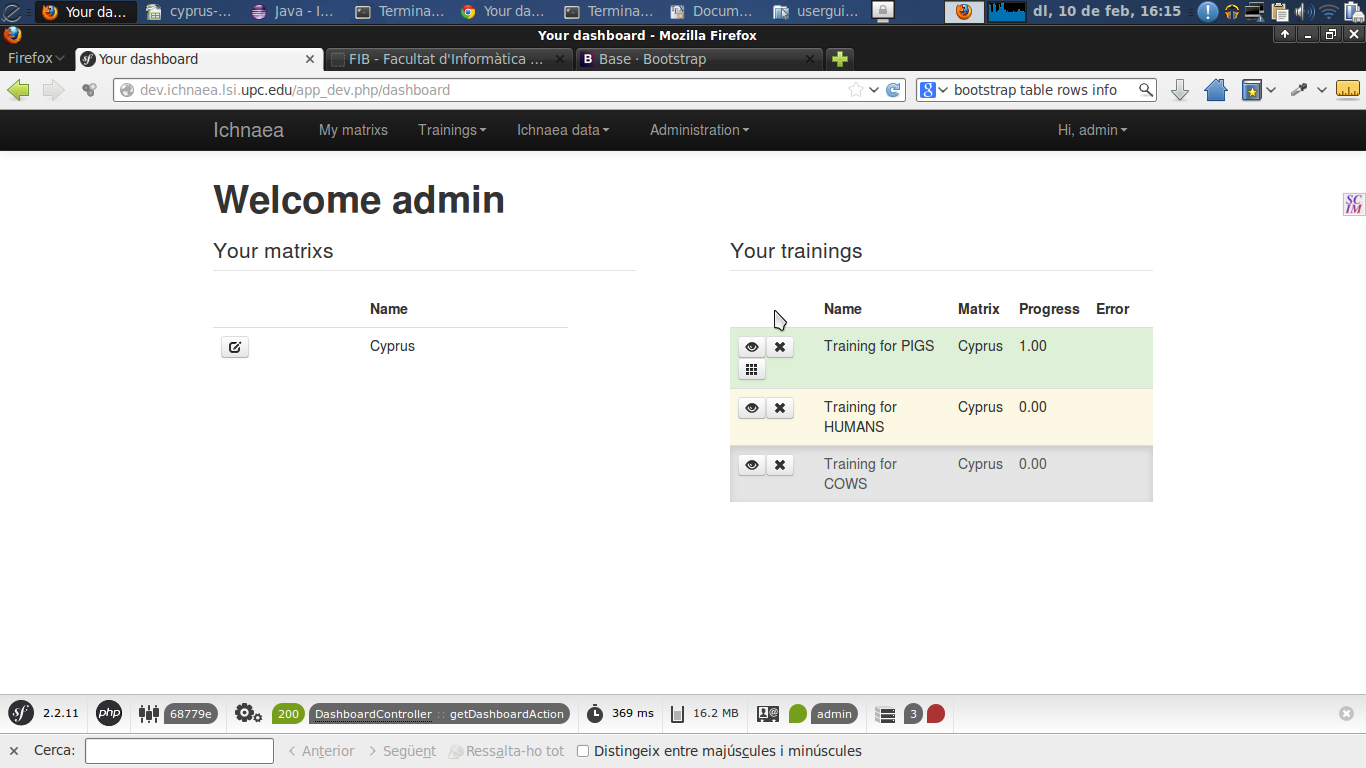
\includegraphics[scale=0.2]{img/userguide/dashboard_complete_trainings.png}
  \caption{Casa de l'usuari}
  \label{fig:placement}
\end{figure}
A continuaci\'{o} descriurem cadascuna de les parts.

\subsection{Llistat dels meus trainings pendents}
Al llistat superior pots veure els trainings que has creat on::
\begin{itemize}
\item Nom de la matriu com a enllaç per veure la matriu
\item Descripci\'{o} del ''training''
\item Data de creaci\'{o}
\item Nom de l'usuari que la creat
\item Progr\'{e}s: actualment Ichnaea no retorna estat del proces. Solament ens diu si ha acabat o no. Per tant els \'{u}nics valors son 0.00 i 1.00.
\item Status. Els possibles status son ''pending''(no s'ha pogut enviar),''sent''(s'ha enviat a la cua) i ''finished''(ha terminat)
\item 
\item Operacions
 \begin{itemize}
 \item ICON_EYE_OPEN es per anar a la pantalla de visualitzaci\'{o} del training.
 \end{itemize}
\end{itemize}

\subsubsection*{Estat del trainings}
En la figura es contempla els estats possibles:
\begin{itemize}
\item Color verd: training sense errors i predectible
\item Color gris: training actualment corrent
\item Color salm\'{o}: ''training'' no s'ha enviat per algun problema amb la cua o amb errors.
\end{itemize}

\section{Variables}
\subsection{Veure les variables del sistema}
Desde el menu ''Ichnaea  Data - View Variables'', es poden veure totes les variables del sistema. Fent click a la icona de edici\'{o}, es pot accedir a la interficie de configuraci\'{o} de la variable seleccionada.

\subsection{Formulari de edici\'{o} d'una variable}
\begin{figure}[h!]
  \centering
  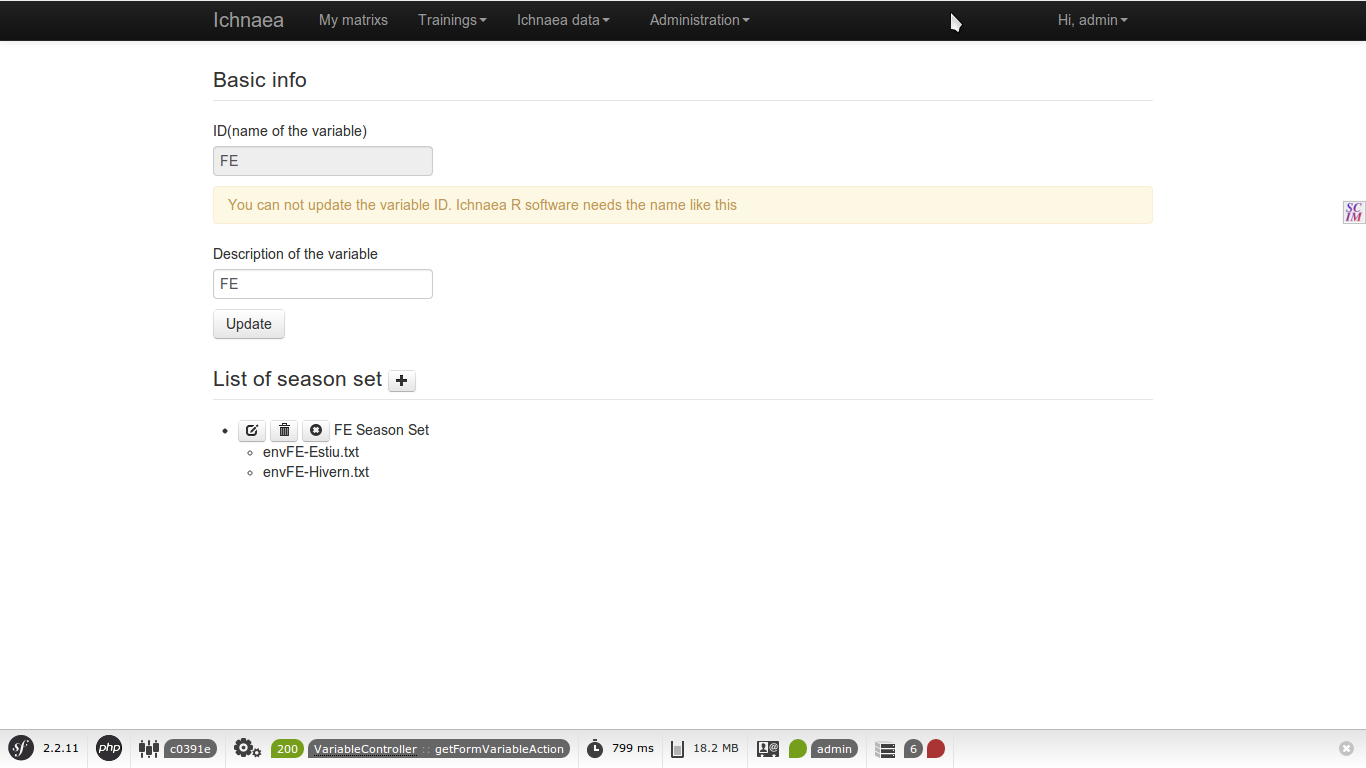
\includegraphics[scale=0.2]{img/userguide/variable_configuration.png}
  \caption{Configuraci\'{o} de variable}
  \label{fig:placement}
\end{figure}
Desde la interf\'{i}cie de configuraci\'{o} es pot:
\begin{itemize}
\item Modificar la descripci\'{o}
\item Accedir a la vista per afegir una ''Season set'', amb la icona del signe de suma.
\item Editar una ''Season Set'', amb ICON_EDIT.
\item Esborrar una ''Season Set'', amb la ICON_TRASH.
\end{itemize}

\subsection{Crear una ''season set'' d'una variable}
\label{season_set:variable}
Per tal de crear un conjunt de seasons per una variable:
\begin{itemize}
\item Llistar les variables per seleccionar una variable('Ichnaea Data - View variables')
\item Editar la variable a la que es vol afegir la variable, fent click ICON_EDIT
\item Al apartat inferior ''List of season set'', clickar a la ICON_PLUS.
\end{itemize}
Es poden donar un nom i afegir tants fitxers com es vulguin. S'ha de tenir cura perque existeix la possibilitat de afegir varis fitxers amb una mateixa configuraci\'{o} (estaci\'{o}). Actualment Ichnaea solament processa estiu e hivern. Per m\'{e}s descripci\'{o} d'aquesta interf\'{i}cie anar al punt \ref{season_set:edit}

\subsection{Editar una ''Season Set'' d'una variable}
\label{season_set:edit}
\begin{figure}[h!]
  \centering
  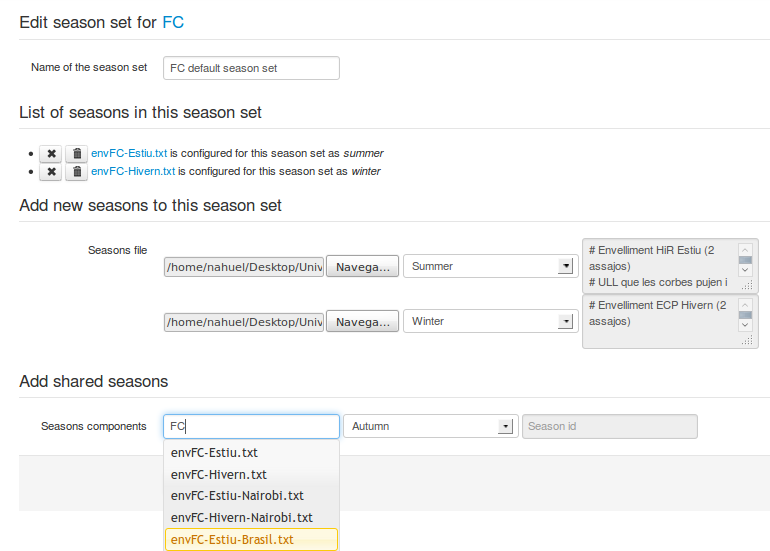
\includegraphics[scale=0.2]{img/userguide/season_set_edition.png}
  \caption{Edici\'{o} de una ''Season Set''}
  \label{fig:placement}
\end{figure}
Desde aquesta vista es pot:
\begin{itemize}
	\item Editar el nom de la season set
	\item Eliminar simplement la relaci\'{o} amb una season amb la icona de la brossa.	
	\item Eliminar un fitxer de la ''Season Set'' i la relaci\'{o}, amb la icona de la creu	
\end{itemize}
S'ha de tenir cura perque exiteix la possibilitat de afegir varis fitxers a una mateixa estaci\'{o}. Actualment Ichnaea solament processa estiu e hivern.

\subsection{Afegir una ''season'' a una ''season set'' existent d'una variable}
Per tal de crear un conjunt de seasons per una variable:
\begin{itemize}
\item Llistar les variables per seleccionar una variable('Ichnaea Data - View variables')
\item Editar la variable a la que es vol afegir la variable, amb ICON_EDIT
\item Editar, amb ICON_EDIT, la ''season set'' del llistat ''List of season set''.
Llegir el punt \ref{season_set:edit}


\section{Matrius}
\subsection{Crear una matriu desde un fitxer csv o excel}
\label{sec:create_matrix}
Desde el menu superior ''IchnaeaData - New matrix'', es pot pujat una nova matriu en format csv o Microsoft Excel. El format csv es compatible amb les programaris de ofim\`{a}tica m\'{e}s habituals como Microsoft Excel o Libreoffice.
El format de la matriu \'{e}s important que sigui el següent.
\begin{center}
    \begin{tabular}{ | l | l | l | p{5cm} |}
    \hline
    Cel.la buida & Alias de la columna & .... & ORIGIN \\ \hline
    Nom de la sample & Valor de la sample  & .... & Origen de la sample \\ \hline
    S01-10-20        & 0,000145            & .... & Human \\ \hline
    \hline
    \end{tabular}
\end{center}
On:
\begin{itemize}
\item Alias de la columna: \'{e}s un nom qualsevol per identificar la columna. Si el sistema cont\'{e} una variable amb el mateix nom, autom\`{a}ticament li assignar aquesta variable amb una ''season set'' per defecte. Si l'alias de variable definit al full de c\`{a}lcul \'{e}s el mateix que el d'una variable del sistema, s'assigna a la variable i li assignar un conjunt de fitxers per defecte.
\item Valor de la sample: \'{e}s el valor de la mostra per la columna(variable)
\item Nom de la sample: \'{e}s un identificador de la mostra. La aplicaci\'{o} mapeja el contingut de subcadenas amb:
\begin{itemize}
\item PL - POULTRY
\item HM - HUMAN
\item PG - PIG
\item CW - COW
\end{itemize}
\item Origen de la sample: \'{e}s una cadena de caracters que especifica l'origen de la mostra. Solament es distingir\'{a} si a les capçaleres a la ultima columna s'especifica la paraula ORIGIN.
\end{itemize}
En la pantalla, es pot seleccionar un fitxer csv i pujar'ho. Seguidament, es podr\`{a} establir la relaci\'{o} de la variable real de la columna i quin conjunt de fitxers per defecte usa. Mirar \ref{sec:configure_matrix}.

\section{Configurar una matriu}
\label{sec:configure_matrix}
Per accedir a configurar una matriu, has d'anar a la teva pantalla de inici(mirar \ref{sec:home}). 
Desde la interficie de configuraci\'{o} es pot configurar:
\begin{itemize}
\item Donar un alias a la columna
\item Asociar una columna a una variable
\item Seleccionar un conjunt de fitxers de la variable
\item Donar nom a una mostra
\item Donar una data a una mostra
\item Donar un origen a un sample
\item Visualitzar missatges de validacions i notificacions
\item Donar acc\'{e}s als usuaris per que puguin crear trainings.
\end{itemize}
\begin{figure}[h!]
  \centering
  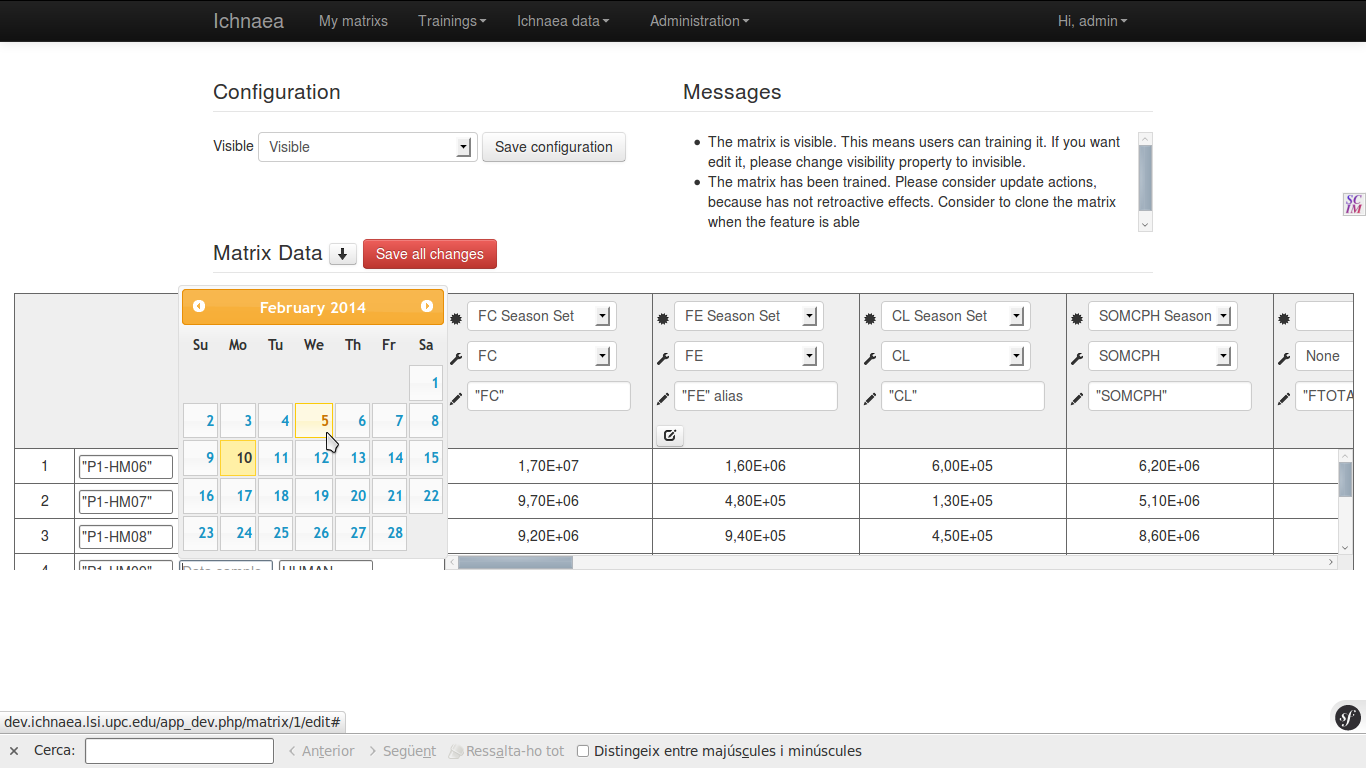
\includegraphics[scale=0.2]{img/userguide/matrix_configure.png}
  \caption{Interficie de configuraci\'{o} de matrius}
  \label{fig:configure_matrix}
\end{figure}

\subsection{Alias de una columna} 
A la secci\'{o} de les capçaleres, a la icona del llapis, es pot especificar un alias a la columna. Si es prem "Enter" o es canvia el focus, s'activa el bot\'{o} de salvaguardat.

\subsection{Especificar una columna a una variable i la season set}
A la secci\'{o} de les capçaleres, a la icona de la clau anglesa, es pot seleccionar la variable del sistema. Autom\'{a}ticament, a la llista de dalt, es carrega la llista de "Seasons Set". Quan es selecciona un dels dos llistats, s'activa el bot\'{o} de salvaguardat. No \'{e}s obligatori donar-li una variable i una "Season Set".

\subsection{Cambiar la visualitzaci\'{o}}
A la secci\'{o} de configuraci\'{o}, es pot cambiar la visibilitat. Si la matriu \'{e}s invisible, els usuaris no poden crear ''trainings''. Per guardar els canvis, s'ha de pitjar el but\'{o} "Save configuration".

\subsection{Visualitzar missatges}
Existeixen diverses restriccions i missatges:
\begin{itemize}
\item Notificaci\'{o} de visibilitat: una matriu visible es entrenable. 
\item Notificaci\'{o} de matriu amb trainings creats. Una modificaci\'{o} crea una incoherencia amb aquests trainings ja que no ser\'{a} la mateixa matriu.
\item Notificaci\'{o} d'origens. Les mostres necessiten obligatoriament uns origins.
\end{itemize}

\subsection{Actualitzar una dada d'una fila i d'una columna}
Es poden actualitzar les dades d'una mostra i d'una 

\section{Clonar una matriu}
\label{sec:clone_matrix}
Desde el menu ''Ichnaea Data - View Matrix'', podem accedir al llistat de variables del sistema. Amb la icona etiquetada com "Clone the matrix", podem clonar una matriu sencera configurada. No es copien els trainings.
\begin{figure}[h!]
  \centering
  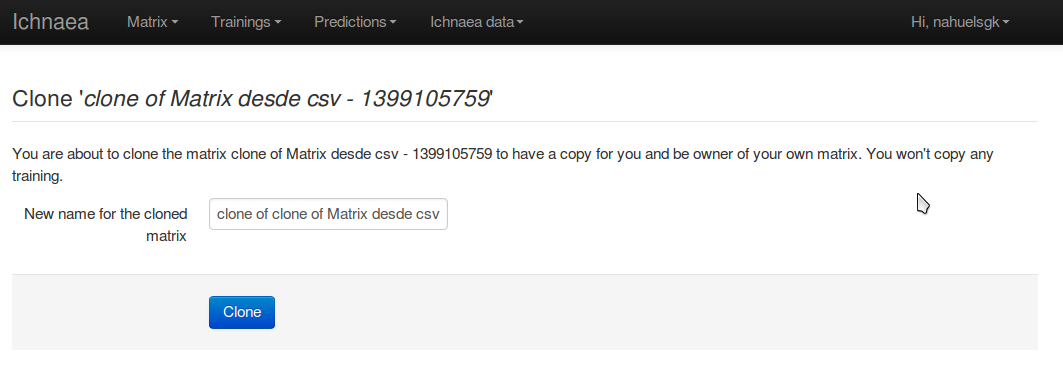
\includegraphics[scale=0.2]{img/userguide/clone_matrix.png}
  \caption{Llistat de matrius}
  \label{fig:placement}
\end{figure}
Fent click a la icona de reload, anem al formulari que suggereix un nom per identificar-la.
\begin{figure}[h!]
  \centering
  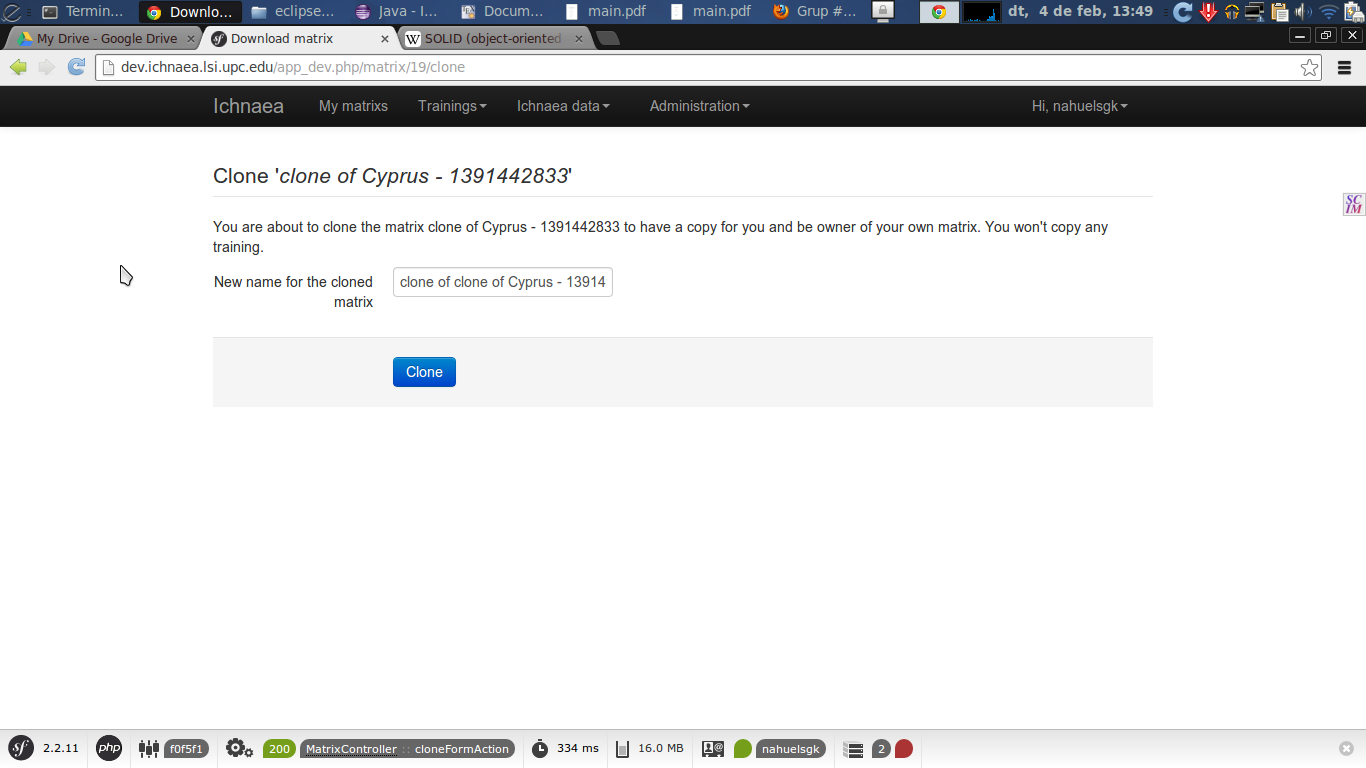
\includegraphics[scale=0.2]{img/userguide/clone_matrix-2.png}
  \caption{Llistat de matrius}
  \label{fig:placement}
\end{figure}
Acceptant, es clona la matriu i anem a la interficie de configuraci\´{o}. Mirar \ref{sec:configure_matrix}.

\section{Crear un training d'una matriu}
Per crear un training s'ha de accedir al menu superior ''Trainings - Create a training''. Desde el llistat de matrius del sistema, amb la icona ICON_ROAD, es pot accedir al formulari de creaci\'{o} de trainings.
\begin{figure}[h!]
  \centering
  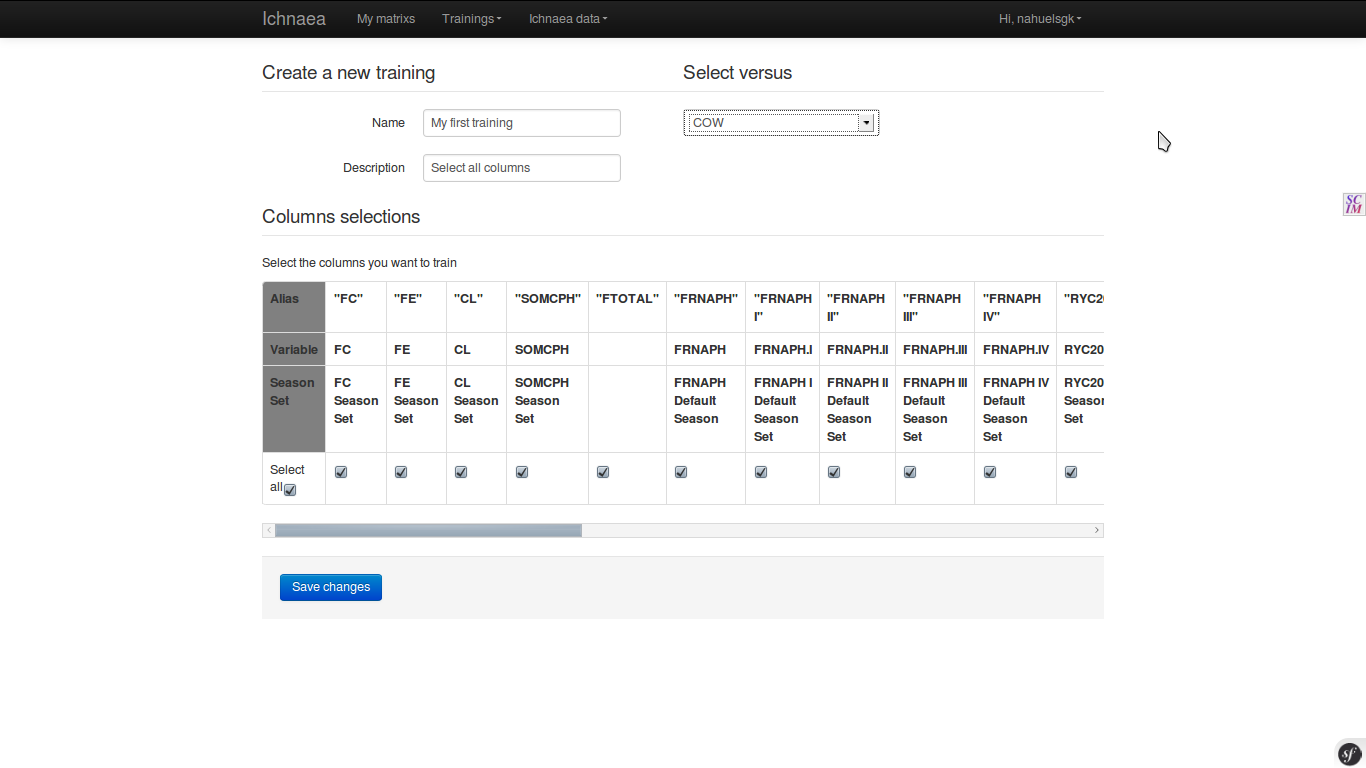
\includegraphics[scale=0.2]{img/userguide/training_create.png}
  \caption{Llistat de matrius}
  \label{fig:placement}
\end{figure}
\begin{itemize}
\item Part esquerra superior: El training cont\'{e} un nom i una descripci\'{o}. Es poden seleccionar quines columnes vols entrenar de la matriu. 
\item Part dreta superior: Desplegable per seleccionar un dels origens disponibles.  El origen-versus, es un llistat de la variable origen de la matriu. Si es selecciona el valor "All versus all", el training ser\'{a} tots contra tots. Si \'{e}s selecciona un origen concret, el training es far\`{a} aquest origen contra els altres. Actualment Ichnaea no suporta aquesta part per\'{o} en el futur est\`{a} planificat que ho far\`{a}.
\item Selecci\'{o} de columnes. Selecci\'{o} de columnes que vols entrenar.
\end{itemize}

Si la creaci\´{o} \´e{s} correcte, les dades s'enviaran a la cua de procesos i la aplicaci\´{o} es redirigir\´{a} la pantalla de visualitzaci\´{o} de trainings.

\subsection{Simular un training de la matriu Cyprus}
Actualment la aplicaci\'{o} Ichnaea i el sistema de cues no esta implantat. Tenim la opci\'{o} de tenir una matriu entrenada en un altre plataforma per poder fer proves amb les interficies de prediccions. Pendent d'implementaci\'{o}.

\section{Visualitzar un training}
Desde la casa de l'usuari(mirar \ref{sec:home}), es pot veure els teus trainings i en quin estadi es troben. Amb la icona "ull", pots accedir a visualitzar la informaci\´{o} del training.

\subsection{Problem\'{a}tiques de la creaci\'{o} de trainings}
\subsubsection*{Error en el enviament}
\begin{figure}[h!]
  \centering
  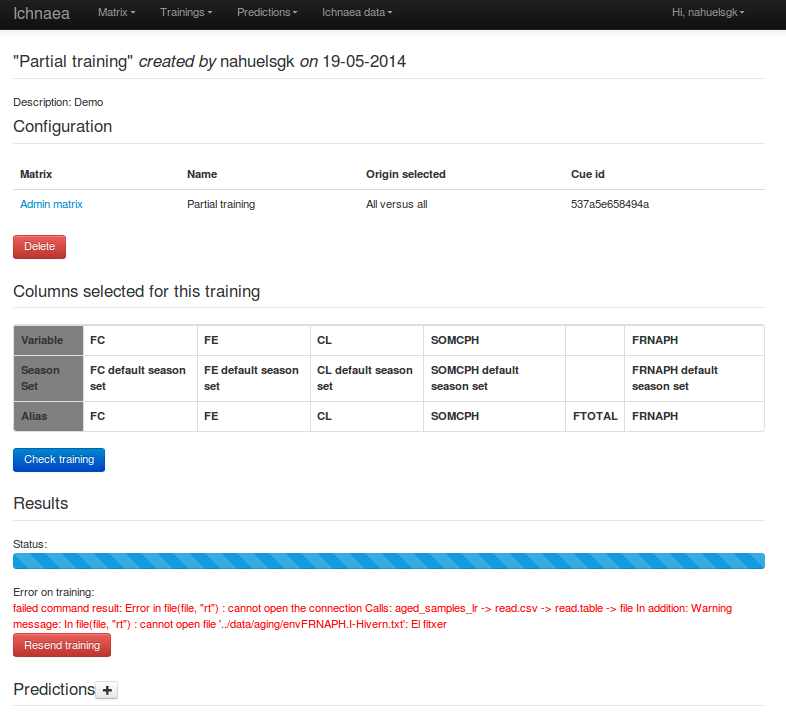
\includegraphics[scale=0.2]{img/userguide/view_training_pending.png}
  \caption{Training que es pot enviar a la cua}
  \label{fig:placement}
\end{figure}

Actualment Ichnaea Software i el sistema de cues no esta implantat. Per defecte, la creaci\'{o} donar\'{a} error. Per tant, es pot utilitzar la simulaci\'{o} de trainings.
A banda d'aix\'{o}, tenim predifinits un conjunt de situacions que a continuaci\'{o} descrivim.

\section{Crear una matriu de predicci\'{o}}
Desde la casa de l'usuari, es pot veure els teus trainings i en quin estadi es troben. Amb la icona "Quadradets"

\section{Crear una predicci\'{o}}
Desde la casa de l'usuari(mirar \ref{sec:home}) es pot crear una predicci\'{o} d'un training. Seleccionant la icona ''quadricules'' de un trainig correcte(en color verd), es pot crear un matriu de predicci\'{o}.

\begin{figure}[h!]
  \centering
  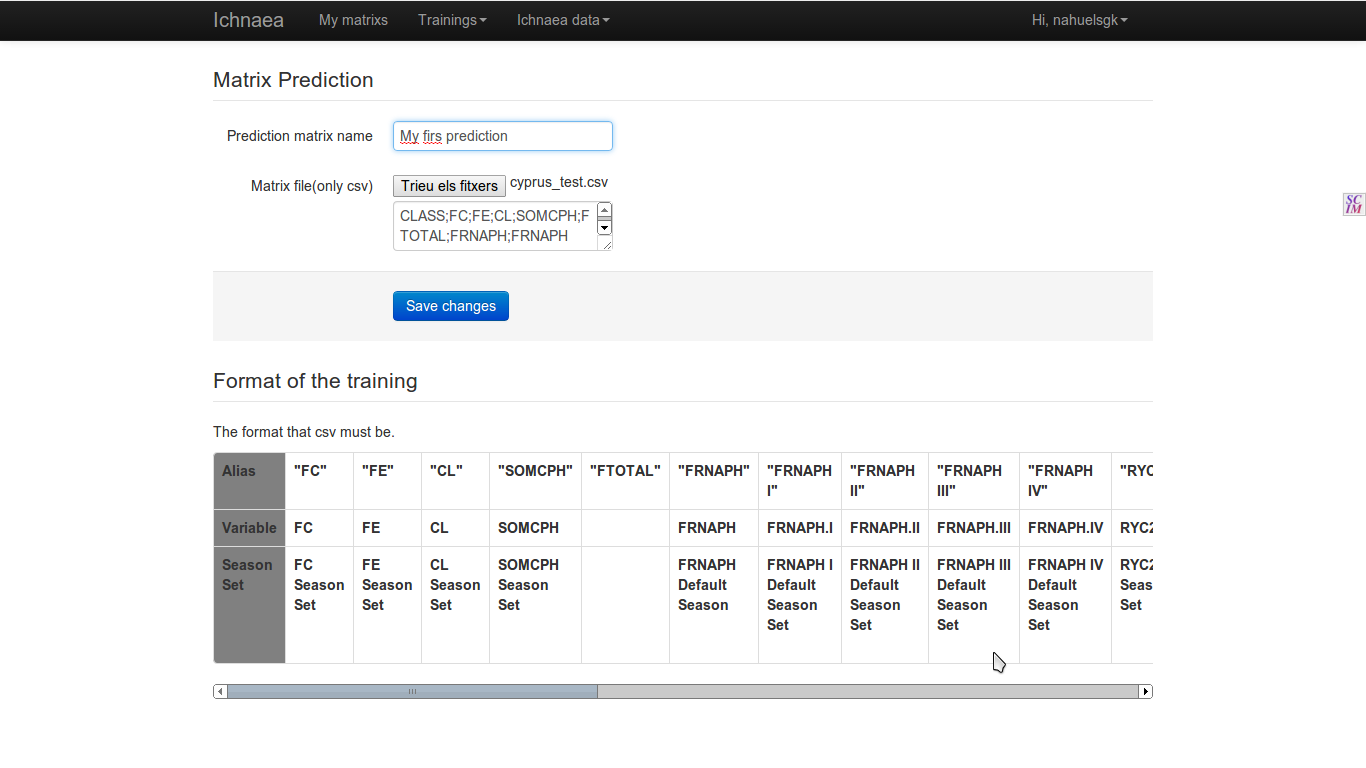
\includegraphics[scale=0.2]{img/userguide/prediction_create.png}
  \caption{Exemple de creaci\'{o} de predicci\'{o}}
  \label{fig:placement}
\end{figure}

A part superior \'{e}s pot seleccionar un fitxer per pujar la matriu per predir. A la part inferior es pot veure les columnes que el training t\'{e} seleccionades. La matrius en format csv ha de tenir el format indicat per la part inferior. En breu es podr\'{a} descarregar una template per tenir el template i poder simplement omplir els valors:
\begin{center}
    \begin{tabular}{ | l | l | l | p{5cm} |}
    \hline
    Cel.la buida & Alias de la columna & .... & ORIGIN \\ \hline
    Nom de la sample & Valor de la sample  & .... & Origen de la sample \\ \hline
    S01-10-20        & 0,000145            & .... & Human \\ \hline
    \hline
    \end{tabular}
\end{center}
Seguidament es pot visualitzar

\section{Actualitzar una matriu de predicci\'{o}}

\section{Llistar les meves prediccions}
Desde el menu superior "Prediction - My predictions" pots llistar les teves prediccions.

\section{Visualitzar una matriu de predicci\'{o}}

\subsection{Actualitzar una matriu de predicci\'{o}}

\subsection{Executar una predicci\'{o} de una matriu de predicci\'{o}}


